\documentclass[a4paper,11pt]{article}
%%%%
%%%%
%PACKAGES______________________________________________________________________________________
\usepackage{simplewick} %Allows Wick Notation
\usepackage{slashed} %Allows feynman slash notation 
\usepackage{graphicx} % graphics, pictures, figures
\usepackage{caption}
\usepackage{subcaption}
\usepackage{verbatim} % importing numerical scripts
\usepackage{multicol, float} % placing floats in right places
\usepackage{algpseudocode} % no idea...
\usepackage[utf8]{inputenc}
\usepackage{amssymb} %needed if not using mathdesign
\usepackage{amsmath}
\usepackage[OT1]{fontenc}
\usepackage{lmodern} %gfsartemisia, times, boisik, et cetera
\usepackage{braket} %dirac notation
\usepackage[cm]{fullpage} % for fulpage style
\usepackage{bm} % boldface vectors
\usepackage{float} % placing floats
\usepackage{relsize} % for \mathlarger command
\usepackage{mathrsfs} %?
\usepackage{textgreek} % cb-greek class
\usepackage{sectsty} % for centering sections
\usepackage{textcomp } % for nr. symbol
\usepackage[usenames, dvipsnames]{color} % defining own colors
\usepackage{type1cm} % scalable fonts
\usepackage{lettrine} % larger first letter in paragraph.
\usepackage{listings}
\usepackage{background} % used for top page text
%\usepackage{niceframe} % for old-school double frame
\usepackage{tikz} % figure config/ creation
%\usepackage{bbold}
%\usepackage{swrule} % for fancy line
%\usepackage{pdfpages} % for importing pdf

%%%%
%%%% SET-UP NEEDED FOR FURTHER PACKAGES
%%%%
\definecolor{hyperclrblue}{RGB}{30,90,125} %Definind own color ; blue
\definecolor{hyperclrorng}{RGB}{210,100,45}%Definind own color
\definecolor{hyperclrgreen}{RGB}{60,120,20}%Definind own color
\usepackage[colorlinks = true,
linkcolor = hyperclrblue,
urlcolor = blue,
citecolor = blue,
anchorcolor = blue]{hyperref} % link package
\usepackage{pgfplots} % to plot directly into latex
\pgfplotsset{compat=1.5} % needed forpgfplots
\usepackage{framed, color} % for framing/shaded box
\definecolor{shadecolor}{cmyk}{0,0,0.185,0} % color for shaded box
\usepackage{fancybox}
\usepackage[sc]{titlesec} % title package
%_______________________________________________________________________________________________
%NEW COMMANDS_________________________________________________________________________________
%\renewcommand*{\thefootnote}{$\dagger$} % creating dagger footnote
\newcommand*{\boisik}{\fontfamily{bsk}\selectfont} % change font to boisik command
\newcommand{\wf}{\text{\textpsi}} % defining wavefunctions as cbgreek class.
\newcommand{\bwf}{\text{\textPsi}} % defining Wavefunctions as cbgreek class.
\newcommand{\Q}{\hat{\text{\boisik Q}}} % defining operator-style 'Q'
\newcommand{\nlm}{\ket{n\ell m_\ell}} % defining wavefunctions as cbgreek class.
\newcommand{\nlmz}{\ket{n\ell m_\ell;0}} % defining wavefunctions as cbgreek class.
\newcommand{\nlmt}{\ket{n\ell m_\ell;t}} % defining wavefunctions as cbgreek class.
%_____________________________________________
%\numberwithin{equation}{section} %equations labeled by section
\sectionfont{\centering} % centering sections with 'sectsty'
\subsectionfont{\centering} % centering sections with 'sectsty'
\definecolor{myclr}{RGB}{190,90,20} %Definind own color
\renewcommand{\thesection}{\Roman{section}.} % Roman numerals for sections
\renewcommand{\thesubsection}{\Alph{subsection}} % Roman numerals for subsections
\titleformat{\section}{\large\scshape\centering}{\thesection}{1em}{} % Change the look of the section titles
\titleformat{\subsection}{\normalsize\centering\bfseries}{\thesubsection.}{1em}{} % Change the look of the section titles
\setlength{\columnsep}{0.7cm}
%______________________________________________________________________________________________
%%%%
%%%%_________________________________________________________________________________________
\begin{document}
%%%% TOP PAGE TEXT
{\SetBgContents{ \textit{{\small\textsc{ Ask J. Markestad, Thorbjørn V. Larsen Universitetet i Oslo. \hspace{3.5cm} \textit{\today}}}}}
\SetBgScale{1}
\SetBgColor{black}
\SetBgAngle{0}
\SetBgOpacity{1}
\SetBgPosition{current page.north east}
\SetBgVshift{-1.2cm}
\SetBgHshift{-10.5cm}
%%%% CREATING TITLE HEADER
$$\:$$
\begin{center}
	\vspace{0.2cm}%\boisik
	\fontsize{15}{15}\selectfont \textsc{ Project 5: Studying fat tails with Monte Carlo simulation of financial interactions between homogeneous agents}\\
	%{in}}\\
	\fontsize{13}{13}\selectfont \textsc{Fys $\textnormal{{4150}}$ }\\
	\vspace{0.4cm}
	\fontsize{12}{12}\selectfont {\textsc{ Ask J. Markestad, Thorbjørn V. Larsen }}\\
	\vspace{0.5cm}
\end{center}
%%%%
%%%%
%______________________________________________________________________________________________
%%%%
%%%%
	
%\includegraphics[scale = 0.48]{line}
\rule{\textwidth}{0.3pt}\par
		
%---------------------------------------------------------------------------------------------------------------------------------------
\begin{abstract}
	In this project we look at some simple agent based models for financial transactions and wealth distribution. We base ourselves on the models presented by Marco Patriarca, Anirban Chakraborti, Kimmo Kaski \cite{GibbsVsnon-Gibbs}, which has a savings component in the transactions but random transactions, and the models by Sanchari Goswami, Parongama Sen \cite{AgentBasedModels} which has interaction preferences. We spend some time analyzing the relations the models of \cite{AgentBasedModels} and the lack of information in this paper, make some changes and do in part our own analysis. We reproduce the distributions of said papers, find the power law fit to the tail end of the distributions, as well as plot the variance to see when the steady state is reached and how large fluctuations are present in said steady states. We also produce distributions with different normalizations, which is lacking in ref. \cite{AgentBasedModels}, and show their effect. Lastly we see the interplay between the free parameters of the most complicated models, not only in the distributions but also in the variance plots where we see that some models never quite seem to reach a steady state, or the steady states have massive fluctuations, to the point were they are no longer steady.
	
\end{abstract}



		
\section*{Introduction}

The field of Financial physics can be said to start in 1897 when V. Pareto \cite{Pareto_1897} found from an empirical study of wealth distribution that the higher end of the distribution followed a power law
 \begin{equation}
 w_m \propto m^{-1-\nu}
 \label{powerLaw}
 \end{equation}
with $\nu \in [1,2]$. This will be the criteria by which all our distributions will be measured, as they will then be considered possibly realistic. The goal of our analysis will be more along the line of seeing how simple changes/additions to the interactions change the wealth distribution. An interesting step further would be to take the distributions which we produce and compare with modern empirical distribution using standard statistical analysis tools of physics today such as hypothesis testing and goodness of fit etc. In this project we concern ourselves with producing the distributions. We start with the models of \cite{GibbsVsnon-Gibbs} and \cite{AgentBasedModels}, present the theory of them, analyze the models of  and critic them, produce the distributions ourselves, find their $\nu$ value to check the distributions realism, and compare with their results. We also plot the variance as a function of the possible transactions, allowing us to see when a steady state is reached or if it is even reached. Lastly we also comment on how to expand this project, or what other models could be interesting to look at.





\section*{Theory and Algorithms}

The initial model of \cite{GibbsVsnon-Gibbs} is a simple one. It considers a system where money is conserved, and all transactions are between random pairs of agents with a random amount of the money an agent has to give. So, given a total of N agents you select two randomly, agents i and j with money $m_i$ and $m_j$. There is some transaction such that $m_i \rightarrow m_i'$ and $m_i + m_j = m_i' + m_j'$. The transaction will be described by a randomly generated number $\epsilon$ between 0 and 1 using a uniform distribution. This leads to the relations:

\begin{align}
m_i' &= \epsilon (m_i + m_j) \\
m_j' &= (1 - \epsilon) (m_i + m_j)
\label{model1}
\end{align}

This type of transaction leads to a steady state given by a Gibbs distribution:

\begin{equation}
w_m = \beta e^{-\beta m}
\label{gibbsDistribution}
\end{equation}

with $\beta = \frac{1}{\braket{m}}$. We will assume here and for all further distributions an initial state where all agents start with an equal amount of money $m_0= 1$. This means that the average money for each agent is the initial cash that they have. This also means that the variance in money is given by:

\begin{equation}
\sigma_m^2 = \braket{m^2} - \braket{m}^2 = \frac{1}{N} \sum_i m_i^2 - 1
\label{variance}
\end{equation} 

We will use this variance as a measure of reaching the steady state as this quantity will start at zero for our initial distribution and grow until it fluctuates around the value for the steady state, if a steady state can be reached. \\

The next interaction type of reference \cite{GibbsVsnon-Gibbs} leads to non-Gibbs distributions. Here we introduce a savings component (If we were to consider taxation it would either always go to one specific agent to be the government, or simply just be redistributed equally among all the agents if we like Karl Marx). We introduce this savings component as a free parameter $\lambda$ of the model and implement it as

\begin{align}
m_i' = \lambda m_i + \epsilon(1 - \lambda) (m_i + m_j) &= m_i + \delta m\\
m_j' = \lambda m_j + (1 - \epsilon)(1 - \lambda) (m_i + m_j) &= m_j - \delta m
\label{model2}
\end{align}

with $\delta m = (1-\lambda)(\epsilon m_j - (1 - \epsilon)m_i)$. \\

We move onto the models presented in \cite{AgentBasedModels}. Goswami and Sen propose that one should include a probability for a transaction to take place, so that not all agent pairs has the same likelihood for interacting. They present three such models with different probabilities, where all the transactions are as in eqs. \ref{model1}. Interestingly, they discuss the $\lambda$ model and point out a similarity between the distributions created from said model and the $\gamma$ model, eq. \ref{model4}, that we will talk about in a bit. Of the three models that they present we will look at two of these, the first one being

\begin{equation}
p_{ij} \propto |m_i - m_j|^{-\alpha}
\label{model3}
\end{equation}

with $\alpha > 0$. This is intended to simulate that people of equal means are more likely to interact than people of different net worths. The problem here is that Goswani and Sen does not provide, or comment, on the normalization for this probability. The problem with this is that the importance of the normalization is connected to the amount of money in the system, i.e. the initial money. In the paper, they use randomly distributed money as an initial state, but they do not provide the initial amount. Why does this matter? Well, say you are in the situation that there is a low amount of money in the system. Then the transactions will be small, and while the relative wealth distribution should be the same the actual differences between the money the agents have will generally be small, which for this probability gate would mean most transactions would be accepted and the distribution should tend towards the one of eqs. \ref{model1}. If however, there is a large amount of money in the system then the differences will generally be larger and most transactions will be rejected. Both of these situations are in and off themselves interesting and relevant but when you don't know which situation you are in, or if you normalize to some in between situation, then the distributions do not tell you that much by themselves. The comparison plots between different $\alpha$ value do include relevant data as it tells us something about the important of this probability gate to a degree, however if most moves where accepted to begin with increasing from 1 to 2 does not change the distribution much while the other case gives larger changes to the distribution. And since this information is not provided, recreating the result to confirm is not possible. We have therefore chosen to have the normalization for this probability as a free parameter that we can tweak such that most transactions get probabilities between 0 and 1, though a larger analysis of its importance to the distribution would be a natural next step.\\

The same problem persists in the next model that is presented where we include a component that prioritizes transactions between agents that have interacted before.

\begin{equation}
p_{ij} \propto |m_i - m_j|^{-\alpha}(c_{ij} + 1)^{\gamma}
\label{model4}
\end{equation}

Where $c_{ij}$ is a matrix that counts the amount of interactions. This of course, introduces a new factor that needs to be normalized. Again, we have a similar problem as above, that given several distributions with different $\gamma$ value we can attain some relevant insight into the model but with problems in knowing exactly what the distribution represents and with reproducibility. How much the $c_{ij}$ should increase with for an interaction is an important factor that needs to be considered in congruence with the normalization. The point is that with running up to $10^{10}$ possible transactions this factor can blow up and produce an always accept situation, and just setting a static value as normalization will not scale with the number of possible interactions like it will in the previous case. This means that how much the $c_{ij}$ increases with says something about how fast you are moved back to model \ref{model1}. Our solution is then to dynamically normalize with the largest element of $c_{ij}$

\begin{equation}
\frac{(c_{ij} + 1)^{\gamma}}{(c_{ij}(max) + 1)^{\gamma}} \leq 1
\label{normalization}
\end{equation}

This does ensure that the importance of previous interactions is still included in the model, but we will never be reduced to a previous model simply by the passage of "time". However, how much $c_{ij}$ in increased with for each transaction between a pair still matters. If the value is increased very slightly, then the chances of leaving an interacting pair "behind" is small, while if the increase is large then it only requires a pair being selected a couple of times in quick succession for "unlucky" pairs to be left behind. And both these cases are interesting, and it says something about how much your model should respect "customer loyalty", and should be included to be able to have reproducibility. Given that \cite{AgentBasedModels} does not comment on the normalization it is hard to say if our model with our dynamic normalization is equivalent to theirs, but we proceed with our model as we believe it to be more interesting. 



\subsection*{Algorithms}

Our Github page for the calculations, program files and benchmarks is found on 

\url{https://github.com/ajmarkestad/Fys4150/tree/master/Project5}\\

To simulate these transactions we use the Monte Carlo method. We set up the program such that the function transaction takes in all our free parameter from the models, i.e. number of agents N, $\lambda$, $\gamma$, $\alpha$, the normalization, the max element of $c_{ij}$, and the matrix $c_{ij}$ itself. It also takes in the parameter totaltransactions, which is the number of possible transactions that should occur for each run. This way, we can consider each time the function transaction is called a measurement and do mean values with respect to the relevant number of runs. We further split up the output part of our main loop in two parts, one for what we call initial cycles and then for after. So for the initial cycles we output the variance, eq. \ref{variance} of the money per agent. We do this as a way to check for steady state solution and give us the "time" it requires to reach this steady state. A second benefit of this approach is that we cut out all the runs where we don't have a steady state from the final distribution, leaving us with only relevant data. The parameter initial cycles is a command line variable and has to be chosen appropriately for each run, as the "time" required to reach equilibrium changes for the different models. The Histogram function is, self written and puts the number of agents within a cash range into an appropriate bin, outputting the distribution that we want for each model. When writing to file we normalize with (total runs - initial cycles). The variable moneyBins is a pre-made array which contains the money each bin should represent and does not change in the program, while the numberofBins gives us the desired resolution in money. 

\begin{lstlisting}
for ( int run= 0; run<= total_runs; run++){
 transaction(previous_interaction_counter,agentlist, numberofAgents, idum, 
 total_transactions, lambda, gamma, alpha,normalization, max);
 if(run>= initial_cycles){
  Histogram(Hist, moneyBins, agentlist, numberofAgents, numberofBins);
 }
 else{
  Output_M(numberofAgents,agentlist);
 }
}
\end{lstlisting}

The main component of the code is the function transaction. It contains all the information about all four of the models that we consider. For each possible transaction, i.e. total transaction, we select two agents randomly, agent1 and agent2. We test that these are two different agents and if they are, we proceed with calculating the intermediate quantity normalization intercounter which we use in the transaction probability and to find the max value later on. We then create a random number between 0 and 1, and use the transaction probability as a gate, so if the random number is less than the probability then we proceed with the transaction, if it is greater than we reject the transaction and find two new random agents. If it passes the test then cash is exchanged, we update $c_{ij}$ with 0.01 to ensure that we most likely, do not have any runaway pairs, update normalization intercounter and test if it is larger than the previous max value. Note that with the way the probability gate is set up if the transaction probability is larger then 1 all moves are accepted, hence the importance of the normalization parameter to ensure that probabilities are between 0 and 1.


\begin{lstlisting}
void transaction(double **previous_interaction_counter,double *agentlist,
int agents, long& idum, int total_transactions, double lambda, double gamma,
double alpha, double normalization, double &max)
{
 double cash_exchange;
 double normalization_intercounter;
 double transaction_probability;
 for (int i=0; i<total_transactions; i++)
 {
  int agent1 = (int) (ran2(&idum)*(double)agents);
  int agent2 = (int) (ran2(&idum)*(double)agents);
  double transaction_rate = (double) (ran2(&idum));
  if(agent1!=agent2)
  {
   normalization_intercounter = 
   pow(previous_interaction_counter[agent1][agent2] +1,gamma);
   transaction_probability =  pow(abs(agentlist[agent1]-agentlist[agent2]),-alpha)
   *normalization_intercounter*(normalization/max);
   if (transaction_probability>1){
    transaction_probability=1.0;
   }
   double transaction_random = (double) (ran2(&idum));
   if(transaction_random<transaction_probability){
    cash_exchange = (1-lambda)*(transaction_rate*agentlist[agent1]-
    (1-transaction_rate)*agentlist[agent2]);
    agentlist[agent1]-=cash_exchange;
    agentlist[agent2]+=cash_exchange;
    previous_interaction_counter[agent1][agent2] += 0.01;
    previous_interaction_counter[agent2][agent1] += 0.01;
    normalization_intercounter = 
    pow(previous_interaction_counter[agent1][agent2] +1,gamma);
    if(normalization_intercounter> max){
     max = normalization_intercounter;
    }
   }
  }
 }
}
\end{lstlisting}

\section*{Results}

We begin with a simple system to test how we see that the system goes towards equilibrium. We calculate the variance of the wealth distribution for every run, which in figure \ref{fig:testinit} has 10000 transactions per run. We see that there is a clear leveling off for the variance, and we will interpret and use this as a check that the system is in a equilibrium situation where we start to sample data just after the last data point. We then change gears in figure \ref{fig:simple} where we have just a simple interaction with extra effects that we model. Here we have upped the transactions per run to $2\cdot 10^6$ to and 2000 total runs to gather more data and we see that the log-log curve \ref{fig:Proper_simple_transaction_log} is a very skewed distribution where a few people have much more money than the bulk. We are interested in how this could be affected by introducing various effects to the model and the first we want to look at is the savings model. 

\begin{figure}[H]
	\centering
	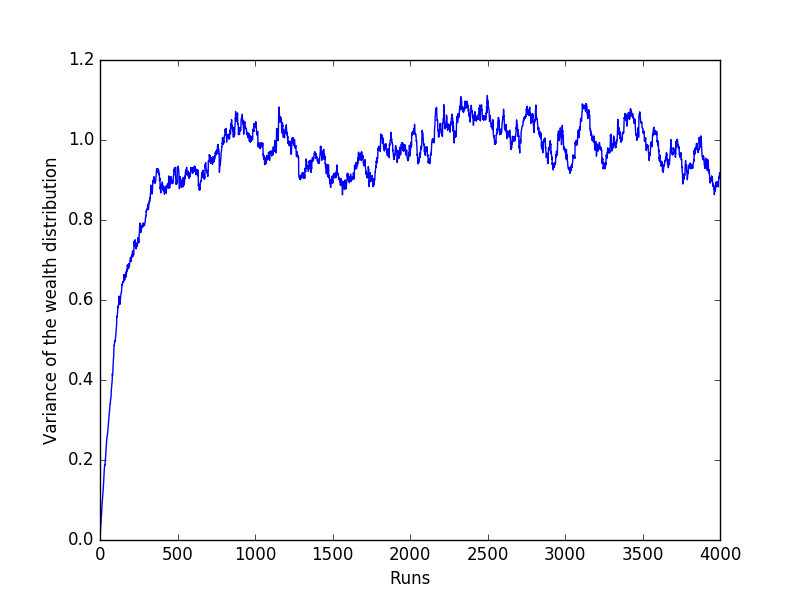
\includegraphics[scale=0.5]{testinit}
	\caption{Variance as the system approaches the equilibrium. We see that the system quickly goes to the equilibrium situation after approximately 10000 transactions.  1000 agents, 10 transactions per run, $\gamma=\alpha=\lambda = 0$,  20000 bins  }
	\label{fig:testinit}
\end{figure}

\begin{figure}[H]
	\centering
	\begin{subfigure}[t]{0.45\textwidth}
		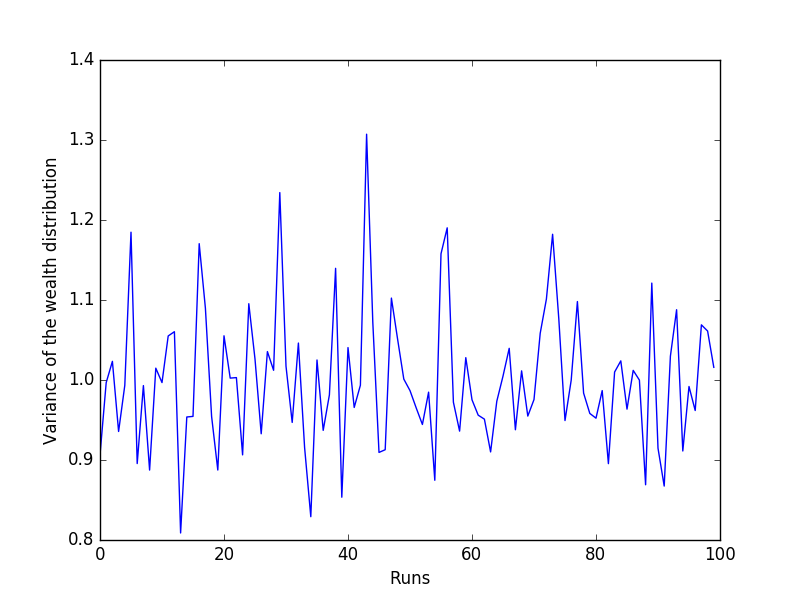
\includegraphics[scale=0.4]{propersimpleinit}
		\caption{Variance of the initial 100 runs, where we see that we get to the equilibrium after the first few run.}
		\label{fig:propersimpleinit}
	\end{subfigure}
	\begin{subfigure}[t]{0.45\textwidth}
		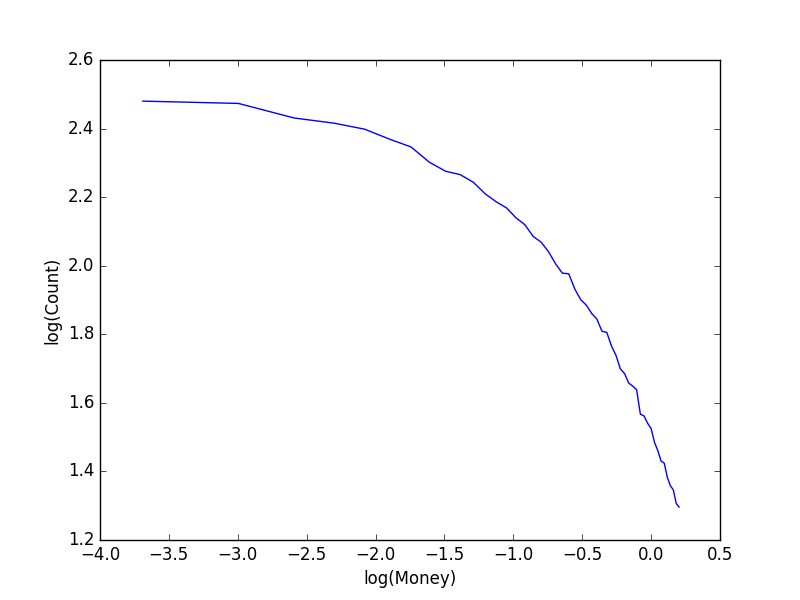
\includegraphics[scale=0.4]{Proper_simple_transaction_log}
		\caption{Loglog plot of the distribution of money. }
		\label{fig:Proper_simple_transaction_log}
	\end{subfigure}
	\caption{Simple transaction, with 500 agens, 2000 total runs, $2\cdot 10^{6}$ transactions per run and  $\lambda=0$, $\alpha=0$, $\gamma=0$, 20000 bins, 100 initial runs, norm = 1.0}
	\label{fig:simple}
\end{figure}







\subsection{Savings models}
As discussed in the theory section, a simplified model of savings is included for each transaction. We see in figure \ref{fig:savings} that this has a big effect on the wealth distribution, where we see that increased savings will give a more even distribution resembling a Gaussian one and less equal to a Gibbs distribution which has a higher frequency of low income persons. We see from figure \ref{fig:savings} the same Gaussian distribution that are portrayed in ref. \cite{GibbsVsnon-Gibbs}.




We can compare this to a power law on the type
\begin{align}
	count (money) = Ax^{-1-\nu} + C
\end{align}
which is equal to the equation in \ref{powerLaw} an use a scipy curve fit to fit the observed data. The method of choosing data for this analysis is given by taking all the data from the first point after the maxima and all the way to the second last non-zero point. For small datasets this will be fairly good as we don't sample as much from the top of the distribution while for large datasets this will inherently give an error as we start the sampling to early. The datapoints that are chosen are the points $[top + (end-top)/3 : end]$ where top is defined as the maxima, and end is defined as the 20'th last nonzero datapoint. We also report uncertainty to get a better handle of the fit. The results are found in table \ref{tab:savings} where we see that we have significantly difference in the power-laws that the distributions follow towards the rich sector. 


\begin{figure}[H]
	\centering
	\begin{subfigure}[t]{0.45\textwidth}
		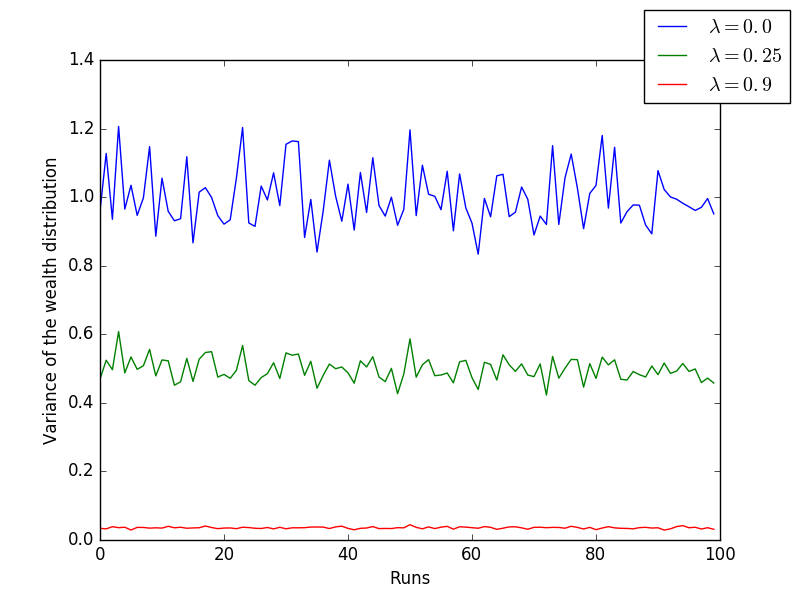
\includegraphics[scale=0.4]{savinginit}
		\caption{Variance of the initial 100 runs, where we see that we get to the equilibrium before we start sampling data}
		\label{fig:savinginit}
	\end{subfigure}
	\begin{subfigure}[t]{0.45\textwidth}
		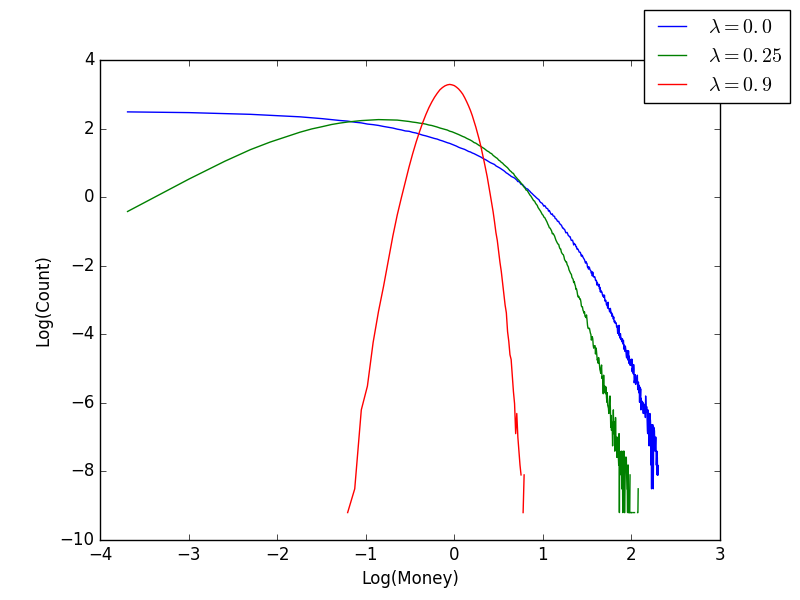
\includegraphics[scale=0.4]{Saving}
		\caption{Introducing a savings amount $\lambda$ affects the wealth distribution of the agents to a large degree where we see that with a higher savings fraction the distribution becomes to a larger degree Gaussian}
		\label{fig:Saving}
	\end{subfigure}
	\caption{Savings models, with 500 agents, 10000 total runs, 100 initial cycles,  $2\cdot 10^{6}$ transactions per run and  $\lambda=[0,0.25,0.9]$, $\alpha=0$, $\gamma=0$,20000 bins, norm = 10.0}
	\label{fig:savings}
\end{figure}

Interesting are the result of the power law fit, suggesting that the savings model gives distributions that do not match with empirical distributions, as mentioned in ref. \cite{AgentBasedModels}.

\begin{table}[h]
\caption{Power law of the tail of the distribution after the maxima. See figure \ref{fig:savings} for parameters}
\begin{center}
\begin{tabular}{c|c|c|c}
$\lambda$ & 0 & 0.25 & 0.9 \\
$\nu$ & $3.74\pm 0.03$ & $4.23\pm 0.04$ & $7.1\pm0.3$
\end{tabular}
\end{center}
\label{tab:savings}
\end{table}%


\subsection{Normalization dependence}
We investigate the effect of the normalization constant we include in our calculations. We use a set of normalizations values $[0.03,0.3,3,30]$ which we run for non-trivial coefficients for all the models we have included in our studies. In figure \ref{fig:norm} we see that we reach the equilibrium quite rapidly but the distribution depends to a great extent of the value we choose. This is because we need to set an upper limit in the probability, and we choose to always accept probabilities that are greater that 1. The scaling with the normalization will affect this such that with a very small normalization all values will be accepted and we won't see any effects of the additional factors we have included(i.e. the nearest neighbor effect). The proper way of handling this is then to have a large normalization constant such that we will see all the relative effects of the underlying models without making any dramatic cuts. The only side-effect of this is that actual transactions will be rare and we therefore have to be careful to check whether our model actually has reached the equilibrium before we start sampling. This choice of a high normalization is reflected in the rest of the results where we chose norm = 10 or norm = 3. 

\begin{figure}[H]
	\centering
	\begin{subfigure}[t]{0.45\textwidth}
		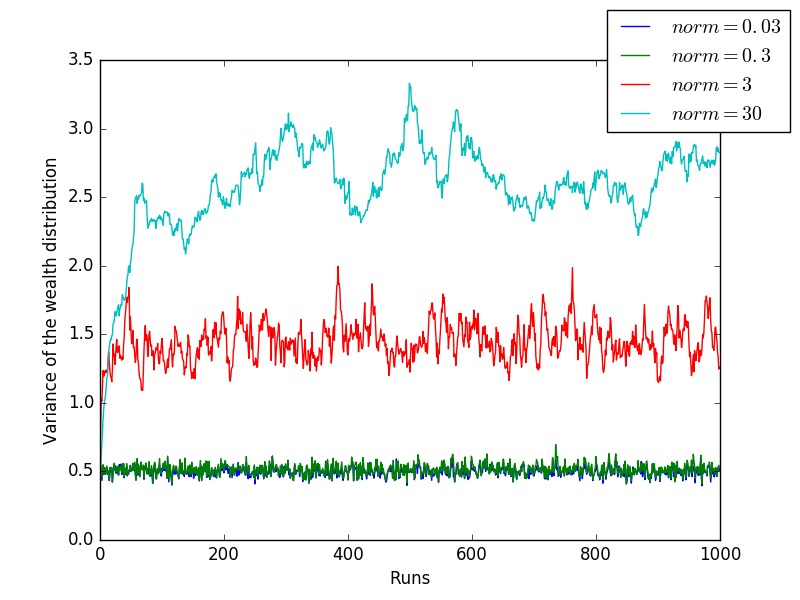
\includegraphics[scale=0.4]{norminit}
		\caption{Variance of the initial 1000 runs, where we see that we get to the equilibrium before we start sampling data}
		\label{fig:norminit}
	\end{subfigure}
	\begin{subfigure}[t]{0.45\textwidth}
		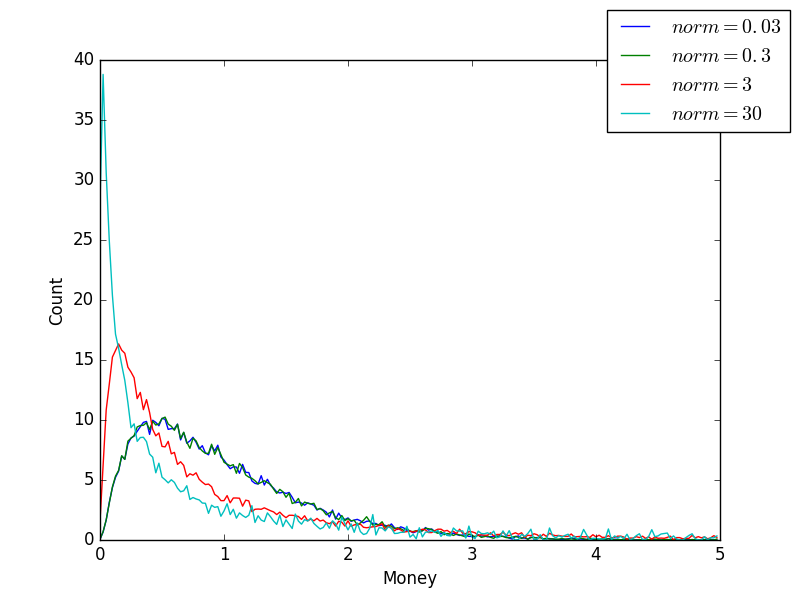
\includegraphics[scale=0.4]{norm}
		\caption{The difference in the normalisation constant has to a large degree an effect in the final outcome of the wealth distribution}
		\label{fig:norm}
	\end{subfigure}
	\caption{Savings models, with 500 agents, 1050 total runs,1000 initial runs,  $2\cdot 10^{3}$ transactions per run and  $norm=[0.03,0.3,3,30]$,$\lambda=0.25$, $\alpha=1$, $\gamma=1$,20000 bins}
	\label{fig:norm}
\end{figure}




\subsection{Nearest neighbor interactions}
People often adapt their spending according to their income, and by this we would expect people with similar income to have a higher probability to interact. As introduced in the theory section we model this effect by a parameter $\alpha$ which increases this effect as we increase the value. We have manually seen that all the simulations have reached equilibrium, so we do not include those plots but present the distributions in figure \ref{fig:alpha_n500} and \ref{fig:alpha_n1000}. Without the savings we see that we are in effect back to the distribution we found in the simple model with the most probable person having no money and increasing the $\alpha$ concentrates the wealth towards the lower end, but with even more people having the least amount of money. If we then look at the models with savings we have a more fair distribution which resembles the Gibbs distribution to a high degree, and if we compare to kinetic theories of gases there is a inverse correspondence between $\alpha$ and the temperature. The power laws that we extract from the observed distributions are reported in table \ref{tab:closepartner} where we see that we clearly get higher $\nu$ values for higher $\alpha$ which coincides with that we see visually. 

\begin{figure}[H]
	\centering
	\begin{subfigure}[t]{0.45\textwidth}
		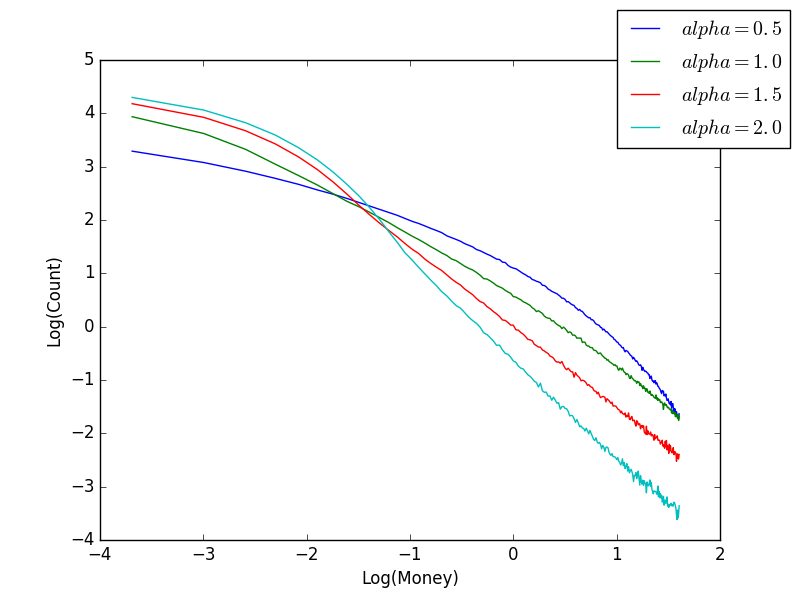
\includegraphics[scale=0.4]{nearestneighbor_lambda=0_0_agens=500}
		\caption{$\lambda = 0.0$, $N=500$}
		\label{fig:0.0_500}
	\end{subfigure}
	\begin{subfigure}[t]{0.45\textwidth}
		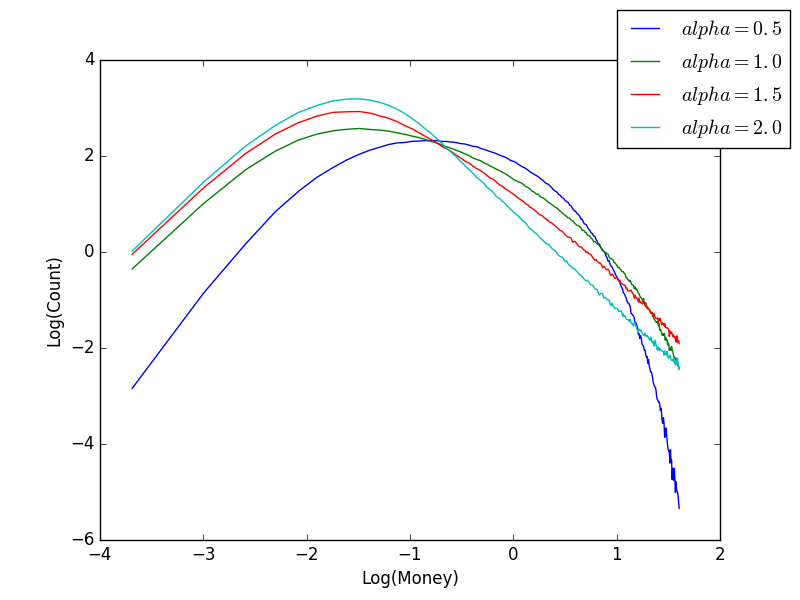
\includegraphics[scale=0.4]{nearestneighbor_lambda=0_5_agens=500}
		\caption{$\lambda = 0.5$, $N=500$}
		\label{fig:0.5_500}
	\end{subfigure}
	\caption{Savings with a nearest neighbor weighted  model, with 500 agents, 5000 total runs,200 initial runs,  $5\cdot 10^{6}$ transactions per run and  $norm=10.0$,$\lambda=[0,0.5]$, $\alpha=[0.5,1.0,1.5,2.0]$, $\gamma=0$,20000 bins}
	\label{fig:alpha_n500}
\end{figure}


\begin{figure}[H]
	\centering
	\begin{subfigure}[t]{0.45\textwidth}
		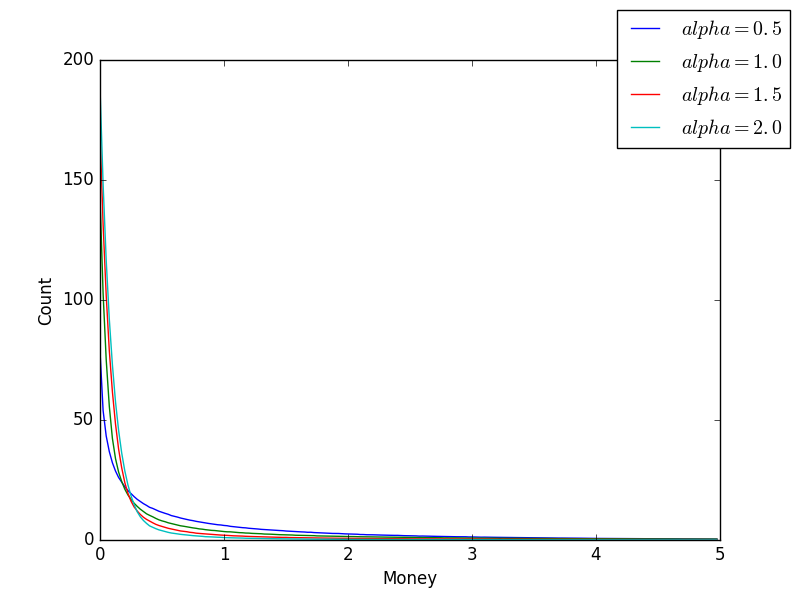
\includegraphics[scale=0.4]{nearestneighbor_lambda=0_0_agens=1000}
		\caption{$\lambda = 0.0$, $N=1000$}
		\label{fig:0.0_1000}
	\end{subfigure}
	\begin{subfigure}[t]{0.45\textwidth}
		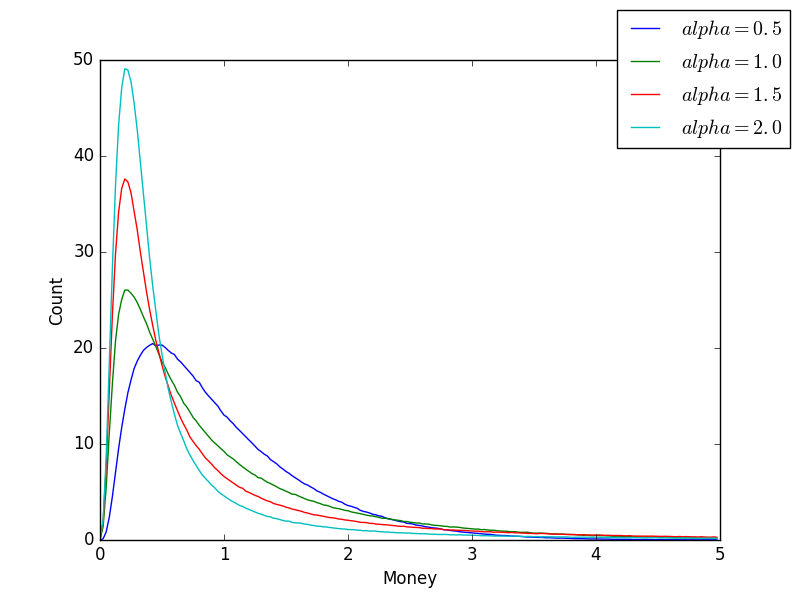
\includegraphics[scale=0.4]{nearestneighbor_lambda=0_5_agens=1000}
		\caption{$\lambda = 0.5$, $N=1000$}
		\label{fig:0.5_1000}
	\end{subfigure}
	\caption{Savings with a nearest neighbor weighted  model, with 1000 agents, 5000 total runs,200 initial runs,  $5\cdot 10^{6}$ transactions per run and  $norm=10.0$,$\lambda=[0,0.5]$, $\alpha=[0.5,1.0,1.5,2.0]$, $\gamma=0$,20000 bins}
	\label{fig:alpha_n1000}
\end{figure}


While we see very little difference in the distributions when we double the number of agents, only a slight increase in all values across the board,but we do see a difference between our distributions and the ones presented in figure 1 of ref \cite{AgentBasedModels}. Of course, ref \cite{AgentBasedModels} uses a $\lambda = 0$ model for their data and we see that the plot has a lot of the same behavior as our equivalent plot, with some significant changes. The point where the models intersect is shifted to around $\sim -1.5$ in our data from $\sim 10$ in theirs. Also, our $\alpha$ distributions all end at the same point while theirs end at different points, notably their $0.5$ value ends first while ours has the largest value for high money amounts. As previously state, ref \cite{AgentBasedModels} does not provide us with enough information to reproduce their results. We note that they normalize with the with the number of agents as well, which we don't and they plot longer in the x axis, however the curves should still match if we had the same normalization of the probability and initial conditions, which they fail to provide. So instead of trying parameters until we make the plots fit, we decided to work with parameters that we felt gave a good spread of these probability values between 0 and 1, as we have done onwards.  


\begin{table}[h]
\caption{See figure \ref{fig:alpha_n500} and \ref{fig:alpha_n1000} for the run-details. The $\lambda=0.0$ and with $\alpha>1$ results in bad line fits as seen in the high uncertainty. }
\begin{center}
\begin{tabular}{c|c|c|c|c}
$\alpha$ & 0.5 & 1.0 & 1.5 & 2.0 \\
$\nu_{N=500, \lambda=0.0}$ & $3.25\pm0.04$ & $2.51 \pm 0.05$ & $0.9 \pm 0.2$ & $1 \pm 2$ \\
$\nu_{N=500, \lambda=0.5}$ & $3.18\pm 0.05$ & $2.57\pm0.03$ & $0.78\pm 0.2$ & $0.2\pm 0.2$  \\
$\nu_{N=1000, \lambda=0.0}$ & $3.51\pm 0.03$ & $2.66\pm 0.05$ & $0.8\pm0.2$  & $0\pm 2$ \\
$\nu_{N=1000, \lambda=0.5}$ & $3.64\pm0.05$ & $2.84\pm 0.04$ & $2.10\pm 0.04$ & $0.7\pm 0.3$ 
\end{tabular}
\end{center}
\label{tab:closepartner}
\end{table}%







\subsection{History of earlier interactions}
We also know that customers tend to not be that exploratory in which brands they buy, and usually stick with the same counter-party and the bond increases over time.  Again as explained in the theory section we can control this effect with a $\gamma$ parameter and we have used instead of an addition of 1 as suggested in the project details we used the value 0.01 to get a more continuous change in the parameter $C_{ij}$. When running this for over 24 hours we still do not get to equilibrium for certain cases as seen in figure \ref{fig:equi} where we have some strange effects especially in figure a where we see that for $\gamma=4$ we actually have something that looks like a lower activity per possible transaction, which would stem from some pair having so many more transactions that others are normalized out and will rarely transact. This would potentially be self enhancing and would be a type of transition of the system where some agents are left behind, which does in some cases model real world behavior where companies go under. For the b plot we see the same effect for $\gamma=4$ but for the other curves we have some weird equilibrium moves that are very sharp and does not look very much like the noise we have seen earlier when the steady state has been reached. 
\begin{figure}[H]
	\centering
	\begin{subfigure}[t]{0.45\textwidth}
		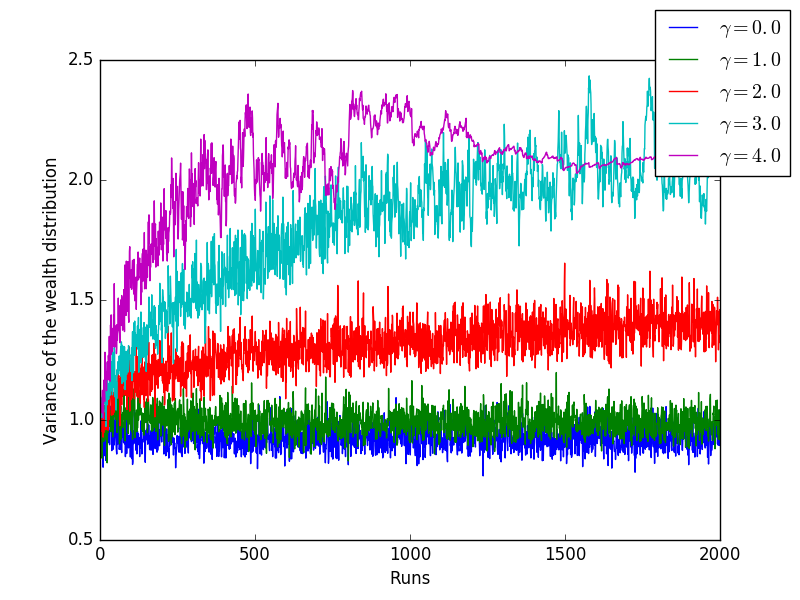
\includegraphics[scale=0.4]{historic_lambda=0_5_alpha=1init}
		\caption{$\alpha=1.0$ }
		\label{fig:historic_lambda=0_0_alpha=1init}
	\end{subfigure}
	\begin{subfigure}[t]{0.45\textwidth}
		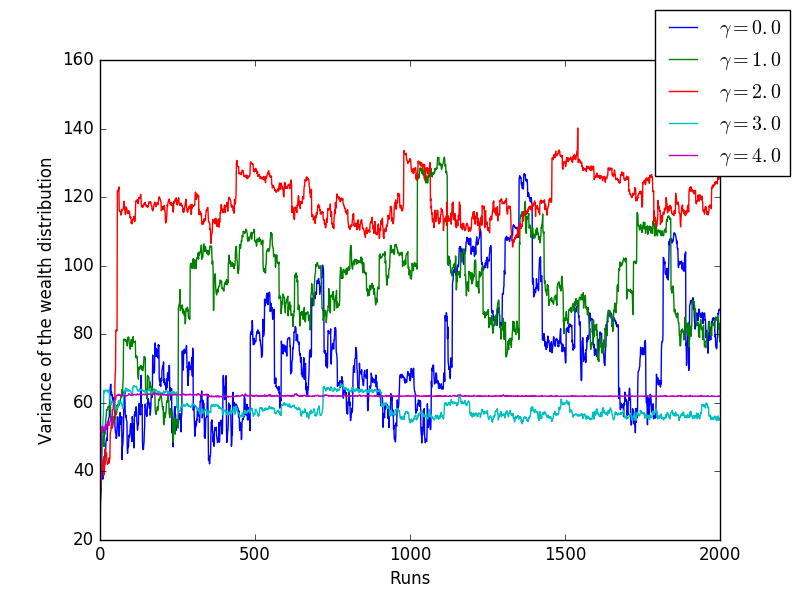
\includegraphics[scale=0.4]{historic_lambda=0_0_alpha=2init}
		\caption{$\alpha=2.0$}
		\label{fig:historic_lambda=0_0_alpha=2init}
	\end{subfigure}
	\caption{Initial variance of the wealth distribution for model with 1000 agents, 10000 total runs,4000 initial runs,  $5\cdot 10^{5}$ transactions per run and  $norm=10.0$,$\lambda=0.5$, $\alpha=[1.0,2.0]$, $\gamma=[0.0,1.0,2.0,3.0,4.0,5.0]$,20000 bins}
	\label{fig:equi}
\end{figure}

We then look at the distributions of wealth in the figure \ref{fig:history_lambda=0_0} and \ref{fig:history_lambda=0_5} where we see the cooling of the system as mentioned above in 9a. Otherwise we see in general that the distributions are similar across the parameter space that we have sampled, with the most important difference is the 9a again where we see that we have a transition from a distribution with a zero count at the lowers money-amount to the maximum at this point. Otherwise the tail-distribution is more interesting to look at and we see in table \ref{tab:hist} that only the models with high $\gamma$ manage to approximately reproduce the experimental data with an appropriate power law, which suggest that such a model with preferred interactions with historic partners might have something to it.  In figure \ref{fig:historic_lambda=0_5_alpha=2} we see some high spikes for the high $\gamma=4.0$ model. Looking at the log(count) value we see that as it is $\approx 0$ an possible explanation is that we have rich people which have stopped to interact with others. 


\begin{figure}[H]
	\centering
	\begin{subfigure}[t]{0.45\textwidth}
		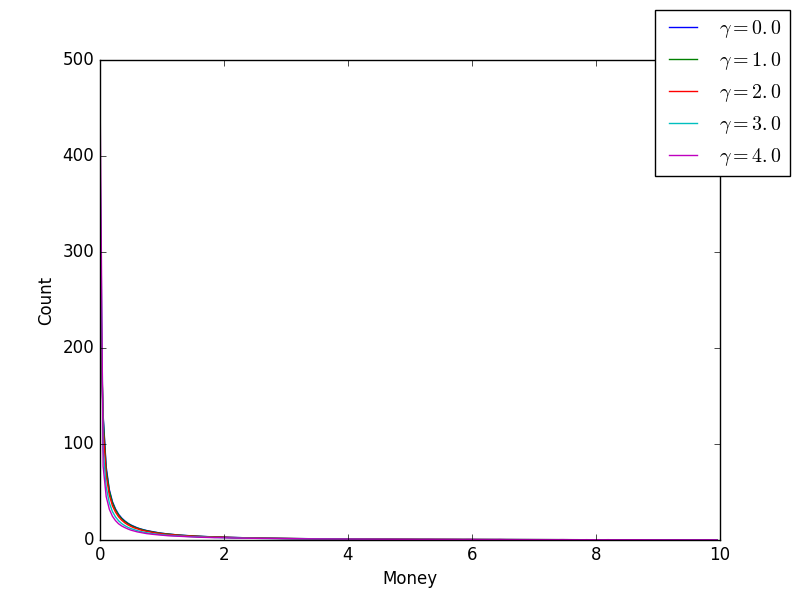
\includegraphics[scale=0.4]{historic_lambda=0_0_alpha=1}
		\caption{$\alpha = 1.0$, $N=500$}
		\label{fig:historic_lambda=0_0_alpha=1}
	\end{subfigure}
	\begin{subfigure}[t]{0.45\textwidth}
		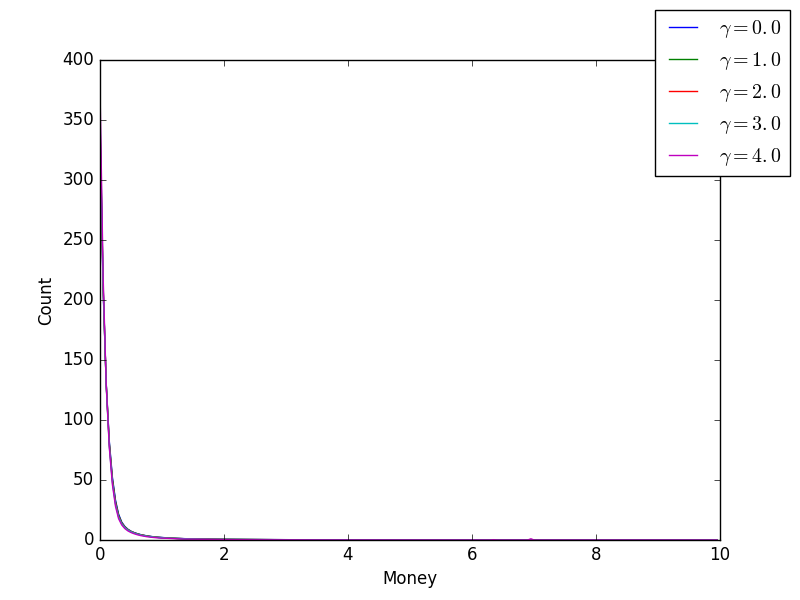
\includegraphics[scale=0.4]{historic_lambda=0_0_alpha=2}
		\caption{$\alpha = 2.0$, $N=500$}
		\label{fig:historic_lambda=0_0_alpha=2}
	\end{subfigure}
	\caption{Savings with a nearest neighbour weighted model which prefers to trade with older trading-partners, with 1000 agents, 10000 total runs,4000 initial runs,  $5\cdot 10^{5}$ transactions per run and  $norm=10.0$,$\lambda=0$, $\alpha=[1.0,2.0]$, $\gamma=[0.0,1.0,2.0,3.0,4.0,5.0]$,20000 bins}
	\label{fig:history_lambda=0_0}
\end{figure}


\begin{figure}[H]
	\centering
	\begin{subfigure}[t]{0.45\textwidth}
		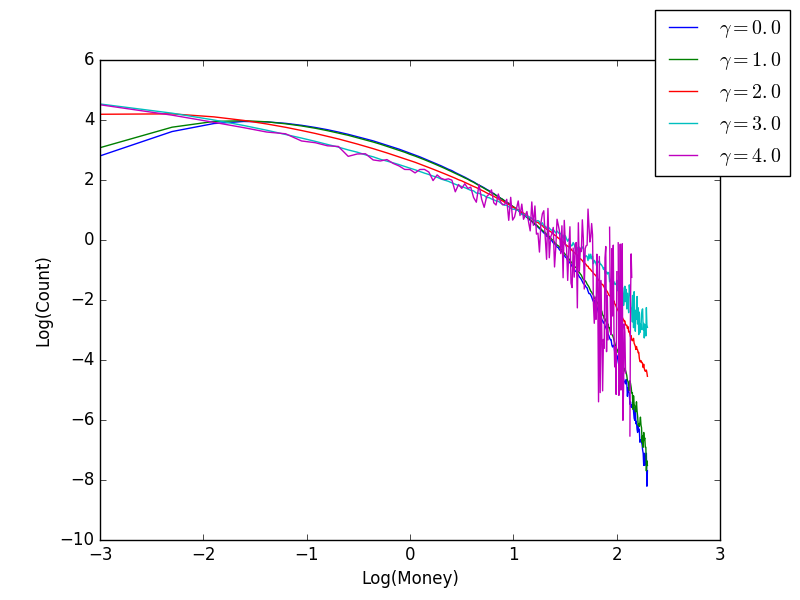
\includegraphics[scale=0.4]{historic_lambda=0_5_alpha=1}
		\caption{$\alpha = 1.0$, $N=1000$}
		\label{fig:historic_lambda=0_5_alpha=1}
	\end{subfigure}
	\begin{subfigure}[t]{0.45\textwidth}
		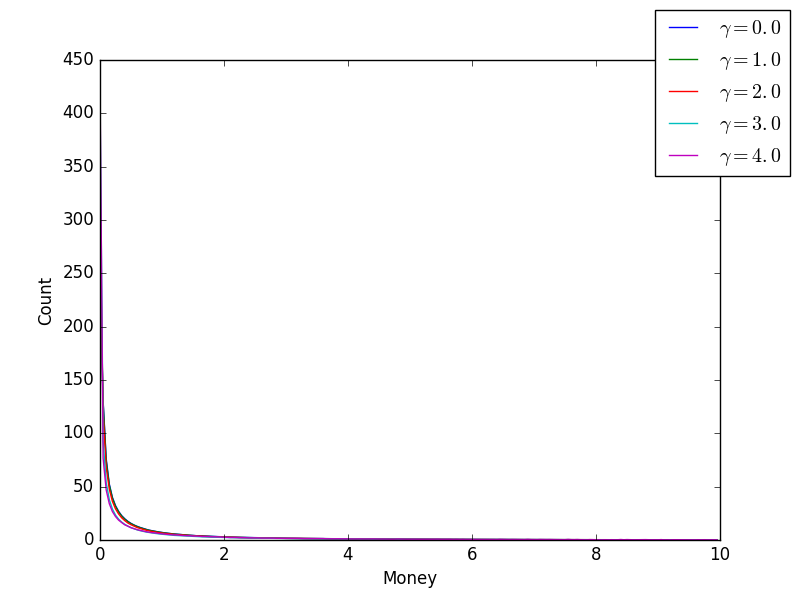
\includegraphics[scale=0.4]{historic_lambda=0_5_alpha=2}
		\caption{$\alpha = 2$, $N=1000$. We see two abnormal peaks in the distribution(see texts for hypotheses)}
		\label{fig:historic_lambda=0_5_alpha=2}
	\end{subfigure}
	\caption{Savings with a nearest neighbour weighted model which prefers to trade with older trading-partners, with 1000 agents, 10000 total runs,4000 initial runs,  $5\cdot 10^{5}$ transactions per run and  $norm=10.0$,$\lambda=0.5$, $\alpha=[1.0,2.0]$, $\gamma=[0.0,1.0,2.0,3.0,4.0,5.0]$,20000 bins}
	\label{fig:history_lambda=0_5}
\end{figure}


\begin{table}[h]
\caption{See figure \ref{fig:history_lambda=0_0} and \ref{fig:history_lambda=0_5} for the run-details}
\begin{center}
\begin{tabular}{c|c|c|c|c|c}
$\gamma$ & 0.0 & 1.0 & 2.0 & 3.0 & 4.0  \\
$\nu_{\alpha=1, \lambda=0.0}$ & $2.85\pm 0.04$ & $3.03\pm 0.04$ & $2.88\pm 0.04$ & $2.48\pm 0.06$ & $1.2\pm0.2$\\
$\nu_{\alpha=2, \lambda=0.0}$ & $-1 \pm 1$ & $-0.4\pm 0.8$ & $0\pm 2$ & $0\pm 3$ & $10\pm 6$ \\
$\nu_{\alpha=1, \lambda=0.5}$ & $2.89\pm 0.05$ & $2.95\pm 0.05$ & $2.57\pm 0.04$ & $1.43\pm 0.08$ &$0.4\pm0.6$  \\
$\nu_{\alpha=2, \lambda=0.5}$ & $3.07\pm 0.03$ & $3.43\pm 0.03$ & $3.01\pm 0.03$ & $2.71\pm 0.05$ & $1.4\pm 0.2$
\end{tabular}
\end{center}
\label{tab:hist}
\end{table}%




\section*{Conclusion}
In our studies we have seen that we are able to simulate agents that make transitions based on different models and get different wealth distributions when making small changes to the mechanisms that underly the interactions. When keeping a simple model we get a Gibbs distribution of the wealth, and if we include a saving in each transaction the distribution becomes a Gaussian one. We then include the preferred interaction(parametrized by $\alpha$) with agents that have similar income and this produces Gibbs distributions(when the saving is non-zero) with a inverse behavior of $\alpha$ wrt temperature in comparison to a kinetic gas model energy distribution. At last we include the effect that interacting with an agents that has previously been interacted with is preferred, and while this has no large effect for the parameters we investigate this can potentially introduce a phase transition where we get the possibility of freezing out agents that never will interact. \\

There are a couple of additions/new models that can be quite interesting to look at for future versions of this project. The obvious is to, as we have done, look deeper into what the normalization of these probability methods means, and unlike us actually have the amount the $c_{ij}$ matrix element increases with as a free parameter as to test its importance contra the $\gamma$ and whether having both as free parameters is superficial. Second is to include a government agent which redistributes its value among the agents either fairly, for a workers utopia, or preferentially of some kind, to the damned bourgeoisie. The first model would most likely not have a tail that fits a power law of the kind one would want for a realistic distribution but it would be a fun exercise. The second one could conceivably give a more realistic distribution and a comparison of these models with some of the simple ones that we have used, capitalist swine we are. Lastly, there is an interesting variant on the $\lambda$ model proposed in \textit{Pareto law in a kinetic model of market with random saving propensity} by Chatterjee et al. \url{http://www.sciencedirect.com/science/article/pii/S0378437103011142}, where they have the value of $\lambda$ be agent specific and distributed between 0 and 1. This means that one recovers the correct tail like behavior for the distribution that is lost with the simpler $\lambda$ model. These \emph{heterogeneous} agents are in contrast to our \emph{homogeneous} agents, and there are many more possible models which potentially could be interesting when this is the case. As a short example we could investigate where in the wealth distribution the different agents tend to end up based on their savings amount.  







\begin{thebibliography}{3}
			
	\bibitem{Pareto_1897}
	V.Pareto
	\emph{Cours d'economie politique}
	1897
	\url{http://www.institutcoppet.org/2012/05/08/cours-deconomie-politique-1896-de-vilfredo-pareto}
	
	\bibitem{GibbsVsnon-Gibbs}
	Marco Patriarca, Anirban Chakraborti, Kimmo Kaski
	\emph{ Gibbs versus non-Gibbs distributions in money dynamics}
	Physica A: Statistical Mechanics and its Applications
	Volume 340, Issues 1–3, 1 September 2004, Pages 334-339, ISSN 0378-4371
	\url{http://dx.doi.org/10.1016/j.physa.2004.04.024.}
	\url{http://www.sciencedirect.com/science/article/pii/S0378437104004327}
	
	\bibitem{AgentBasedModels}
	Sanchari Goswami, Parongama Sen
	\emph{ Agent based models for wealth distribution with preference in interaction}
	Physica A: Statistical Mechanics and its Applications
	Volume 415, 1 December 2014, Pages 514-524, ISSN 0378-4371
	\url{http://dx.doi.org/10.1016/j.physa.2014.08.018.}
	\url{http://www.sciencedirect.com/science/article/pii/S0378437114006967}
	
	
			
			
			
\end{thebibliography}
		
		
		
		
		
		
		
		
		
%__________________________________________________________________________
\end{document}
